\documentclass[11pt]{article}
\ifdefined\pdftrailerid\pdftrailerid{}\fi
\input{glyphtounicode}
\pdfgentounicode=1
\pdfglyphtounicode{parenleftbig}{0028}
\pdfglyphtounicode{parenrightbig}{0029}
\pdfglyphtounicode{bracketleftbig}{005B}
\pdfglyphtounicode{bracketrightbig}{005D}
\pdfglyphtounicode{floorleftbig}{230A}
\pdfglyphtounicode{floorrightbig}{230B}
\pdfglyphtounicode{ceilingleftbig}{2308}
\pdfglyphtounicode{ceilingrightbig}{2309}
\pdfglyphtounicode{radicalbig}{221A}
\pdfglyphtounicode{parenleftBig}{0028}
\pdfglyphtounicode{parenrightBig}{0029}
\pdfglyphtounicode{bracketleftBig}{005B}
\pdfglyphtounicode{bracketrightBig}{005D}
\pdfglyphtounicode{floorleftBig}{230A}
\pdfglyphtounicode{floorrightBig}{230B}
\pdfglyphtounicode{ceilingleftBig}{2308}
\pdfglyphtounicode{ceilingrightBig}{2309}
\pdfglyphtounicode{radicalBig}{221A}
\pdfglyphtounicode{parenleftbigg}{0028}
\pdfglyphtounicode{parenrightbigg}{0029}
\pdfglyphtounicode{bracketleftbigg}{005B}
\pdfglyphtounicode{bracketrightbigg}{005D}
\pdfglyphtounicode{floorleftbigg}{230A}
\pdfglyphtounicode{floorrightbigg}{230B}
\pdfglyphtounicode{ceilingleftbigg}{2308}
\pdfglyphtounicode{ceilingrightbigg}{2309}
\pdfglyphtounicode{radicalbigg}{221A}
\pdfglyphtounicode{parenleftBigg}{0028}
\pdfglyphtounicode{parenrightBigg}{0029}
\pdfglyphtounicode{bracketleftBigg}{005B}
\pdfglyphtounicode{bracketrightBigg}{005D}
\pdfglyphtounicode{floorleftBigg}{230A}
\pdfglyphtounicode{floorrightBigg}{230B}
\pdfglyphtounicode{ceilingleftBigg}{2308}
\pdfglyphtounicode{ceilingrightBigg}{2309}
\pdfglyphtounicode{radicalBigg}{221A}
\pdfglyphtounicode{vextendsingle}{007C}
\pdfglyphtounicode{circleplustext}{2A01}
\pdfglyphtounicode{circleplusdisplay}{2A01}
\pdfglyphtounicode{summationtext}{2211}
\pdfglyphtounicode{summationdisplay}{2211}
\pdfglyphtounicode{producttext}{220F}
\pdfglyphtounicode{productdisplay}{220F}
\pdfglyphtounicode{integraltext}{222B}
\pdfglyphtounicode{integraldisplay}{222B}
\pdfglyphtounicode{logicalandtext}{22C0}
\pdfglyphtounicode{logicalanddisplay}{22C0}
\pdfglyphtounicode{hatwider}{005E}
\usepackage[T1]{fontenc}
\usepackage{lmodern}
\usepackage[utf8]{inputenc}
\usepackage[margin=1in]{geometry}
\usepackage{amsmath,amssymb,amsthm,mathtools}
\usepackage{booktabs,microtype,xcolor,listings,needspace}
\usepackage{tikz}
\usetikzlibrary{arrows.meta,positioning}
\usepackage[colorlinks=true,linkcolor=blue!45!black,citecolor=blue!45!black,urlcolor=blue!45!black]{hyperref}
\hypersetup{pdftitle={A Fock-space inequality and the Laughlin spectral gap},pdfauthor={OpenAI},pdfsubject={The full fermionic V1 interaction on the round sphere},pdfkeywords={Laughlin state, spectral gap, fractional quantum Hall effect, pseudopotential, sphere}}
\newtheorem{theorem}{Theorem}[section]
\newtheorem{proposition}[theorem]{Proposition}
\newtheorem{lemma}[theorem]{Lemma}
\newtheorem{corollary}[theorem]{Corollary}
\theoremstyle{remark}
\newtheorem{remark}[theorem]{Remark}
\newcommand{\FF}{\mathcal F}
\newcommand{\LL}{\mathcal L}
\newcommand{\ran}{\operatorname{ran}}
\newcommand{\tr}{\operatorname{tr}}
\newcommand{\diag}{\operatorname{diag}}
\newcommand{\eps}{\varepsilon}
\newcommand{\ket}[1]{\lvert #1\rangle}
\newcommand{\bra}[1]{\langle #1\rvert}
\newcommand{\ip}[2]{\langle #1,#2\rangle}
\newcommand{\norm}[1]{\lVert #1\rVert}
\lstset{basicstyle=\ttfamily\scriptsize,columns=fullflexible,keepspaces=true,breaklines=true,frame=single}
\title{A Fock-space inequality and the Laughlin spectral gap}
\author{OpenAI}
\date{September 24, 2026}
\AddToHook{env/theorem/before}{\Needspace{4\baselineskip}}
\AddToHook{env/proposition/before}{\Needspace{4\baselineskip}}
\AddToHook{env/lemma/before}{\Needspace{4\baselineskip}}
\AddToHook{env/corollary/before}{\Needspace{4\baselineskip}}
\begin{document}
\maketitle
\begin{abstract}
We prove the spherical fermionic Laughlin spectral-gap conjecture for the
full \(V_1\) interaction. With coefficient one for each pair projector,
the gap above the Laughlin state at filling \(1/3\) on the round sphere
is at least \(1/25\) for all sufficiently large systems.
More generally, \(H_Q^2\ge\gamma H_Q\) for some fixed \(\gamma>1/25\)
on the entire lowest-Landau-level Fock space for all sufficiently large
flux \(Q\), independently of particle number.
\end{abstract}
\section{The gap and the model}
\label{sec:intro}
Laughlin's wave function gave an explicit description of the fractional
quantum Hall state at filling $1/3$~\cite{Laughlin}. Haldane's spherical
geometry and pseudopotentials identify a particularly simple parent
Hamiltonian: every pair pays energy one in relative angular momentum one
and zero in the other pair sectors~\cite{Haldane}. Its exact Laughlin
zero mode is known, but a uniform lower bound on the positive spectrum
requires control of all competing many-particle states. We prove this
bound for the full interaction on the round sphere, resolving positively
the spherical fermionic Laughlin spectral-gap conjecture.

The gap question has accompanied this model since its early development.
Haldane and Rezayi's finite-size study supplied numerical evidence and
explicitly distinguished the expected hard-core gap from a formal
proof~\cite{HaldaneRezayi1985FiniteSize}. The density-wave variational
picture of Girvin, MacDonald, and Platzman explains important features of
the excitation spectrum~\cite{GMP}. A variational excitation energy is
an upper bound; the lower bound sought here must hold for every state
orthogonal to the zero modes.

\subsection{Normalization and main results}
For an integer \(Q\ge1\), let \(U_Q\) be the spin-\(Q/2\) representation of
\(SU(2)\), equipped with its invariant inner product. It is the one-particle
lowest Landau level on the sphere with \(Q\) flux quanta. Equivalently, it is
the space of homogeneous polynomials of degree \(Q\) in spinor coordinates
\((u,v)\). For \(2\le N\le Q+1\), define
\begin{equation}\label{eq:physicalH}
 H_{N,Q}=\left.\sum_{1\le i<j\le N}P_{ij}^{(1)}
          \right|_{\bigwedge^N U_Q},
\end{equation}
where \(P_{ij}^{(1)}\) is the orthogonal projector onto pair spin \(Q-1\)
in tensor positions \(i,j\). This is relative angular momentum one. The sum
preserves the antisymmetric subspace. Each unordered pair has coefficient
one, with no rescaling depending on \(N\) or \(Q\).

Set \(H_{0,Q}=H_{1,Q}=0\), and write
\[
 \FF_Q=\bigoplus_{N=0}^{Q+1}\bigwedge^N U_Q,\qquad
 H_Q=\bigoplus_{N=0}^{Q+1}H_{N,Q},\qquad
 \gamma_*=\frac{4616733319001}{10^{14}}> \frac1{25}.
\]
Our principal estimate concerns this entire Fock space.

\begin{theorem}\label{thm:fock}
For every \(0<\gamma<\gamma_*\), there is an integer \(Q_\gamma\) such that
for every integer \(Q\ge Q_\gamma\),
\begin{equation}\label{eq:architecture}
 H_Q^2\ge\gamma H_Q\qquad\text{on }\FF_Q.
\end{equation}
The threshold \(Q_\gamma\) is independent of particle number.
\end{theorem}

Thus the spectrum is contained in \(\{0\}\cup[\gamma,\infty)\).
In a particle sector without a zero mode, this statement bounds the energy
away from zero; it does not assert a gap between that sector's two lowest
eigenvalues. At Laughlin filling the zero mode is unique, and we obtain the
usual ground-state spectral gap.

\begin{corollary}\label{thm:main}
There is an integer \(N_0\ge2\) such that, for every \(N\ge N_0\) and
\(Q=3(N-1)\),
\begin{equation}\label{eq:main}
 H_{N,Q}\ge\frac1{25}\bigl(I-P_{\mathrm L,N}\bigr)
 \qquad\text{on }\bigwedge^N U_Q,
\end{equation}
where \(P_{\mathrm L,N}\) projects onto the line spanned by
\[
 \Psi_{\mathrm L,N}=\prod_{i<j}(u_iv_j-u_jv_i)^3.
\]
\end{corollary}

At fixed magnetic length, the sphere radius is proportional to \(\sqrt Q\),
so this is the two-dimensional thermodynamic limit. The thresholds in
Theorem~\ref{thm:fock} and Corollary~\ref{thm:main} are existential.
The proof does not give an explicit flux threshold or the endpoint
coefficient \(\gamma_*\) on finite spheres.

\subsection{Prior work}
The exact ground-state structure is an established part of the theory.
Besides Haldane's spherical construction, Trugman and Kivelson obtained
exact Laughlin ground states for repulsive interactions in a vanishing-range
limit~\cite{TrugmanKivelson1985}. The second-quantized algebra of
pseudopotentials was developed systematically by Ortiz, Nussinov, Dukelsky,
and Seidel~\cite{OrtizNussinovDukelskySeidel}. Chen and Seidel, and
Mazaheri, Ortiz, Nussinov, and Seidel, gave algebraic constructions and
characterizations of their zero modes~\cite{ChenSeidel2015,MazaheriOrtizNussinovSeidel2015}.
These results identify the zero modes that a spectral estimate must preserve. We include a short self-contained proof of the known spherical
zero-mode uniqueness at the Laughlin flux in Lemma~\ref{lem:kernel}.

For Laughlin states on a cylinder of any fixed radius, Jansen established
thermodynamic correlation limits and axial periodicity~\cite{Jansen2012}.
Exact ground states of related finite-range orbital chains, including
squeezed and matrix-product states, were constructed by Nakamura, Wang, and
Bergholtz~\cite{NakamuraWangBergholtz2012} and by Wang and
Nakamura~\cite{WangNakamura2013}. Nachtergaele, Warzel, and Young proved
uniform gaps for a truncated fermionic pseudopotential~\cite{NWY};
Warzel and Young obtained thin-torus bounds that separate bulk behavior
from open-chain edge modes~\cite{WY}. Their invariant-subspace method
also treats a truncated bosonic pseudopotential~\cite{WarzelYoung2023BulkEdge}.
The fermionic estimates already hold uniformly across particle sectors.
The distinction in Theorem~\ref{thm:fock} is the full spherical pair
interaction, with its fixed projector normalization and sphere radius
growing in the thermodynamic limit. The finite support used in our
auxiliary comparison operators does not truncate that interaction.

Recent work gives further structural and spectral information.
Lemm, Nachtergaele, Warzel, and Young derive recursions between particle
sectors and compare charge and neutral gaps~\cite{LemmNachtergaeleWarzelYoung2026Recursive};
a uniform bound for the full pseudopotential still requires control of
the model-specific ground-space overlap matrices in those criteria.
Schraven and Warzel prove entanglement-gap and clustering results for
Laughlin states on sufficiently thin cylinders~\cite{SchravenWarzel2026IMPS}.
The entanglement spectrum is distinct from the Hamiltonian spectrum
considered here. Density rigidity within the family of fully correlated
Laughlin states is another complementary form of incompressibility,
established by Lieb, Rougerie, and Yngvason~\cite{LRYRigidity}.
No density-screening assumption enters our argument.

Rougerie's survey records the spectral-gap conjecture and its geometric
formulations~\cite[Appendix~A]{Rougerie}. For $N$ fermions in the planar
lowest Landau level, consider the sum over unordered pairs of the orthogonal
projectors onto relative polynomial degree one, each with coefficient one
and with center-of-mass degree unrestricted. Section~\ref{sec:plane} proves
that its positive spectrum is bounded below by the endpoint $\gamma_*$,
uniformly in particle number $N\ge2$ and total polynomial degree $L$.
In particular, this proves the fermionic cubic case of the folklore
spectral-gap conjecture in \cite[Conjecture~A.1]{Rougerie}, whose degree range
is $L\le3N(N-1)/2$.

\subsection{Proof strategy}
Proving positivity of $H^2-\gamma H$ is a standard route to a gap,
underlying finite-size criteria~\cite{Knabe} and methods based on positive
local decompositions~\cite{Cruz,Rai}. Our argument uses rotations and
angular-momentum decomposition to construct such a comparison.
It starts from the normal-ordered expansion of \(H_Q^2\).
It has two-, three-, and four-body terms. We compare them with the
corresponding terms of a positive operator
\[
 \mathcal K_Q=(2Q-1)\int_{SU(2)}
                  \sum_{\rho=1}^{7}F_\rho(g)^\dagger F_\rho(g)\,dg,
\]
where each \(F_\rho\) is a specified linear combination of a pair
annihilator and operators that annihilate three particles and create one.
Here \(F_\rho(g)\) denotes rotation by \(g\), and Haar measure has mass
one. These auxiliary operators involve finitely many orbital modes;
the Hamiltonian itself is never truncated.

Rotational symmetry reduces the comparison to fixed spin blocks.
The three-body blocks have an explicit spectrum and a summable tail.
For four particles, coupling the interacting pair to the different spin
sectors of a second pair can produce several copies of the same total spin.
Their four-particle images under exterior multiplication can be linearly
dependent.
For the retained blocks, seven rows of rational data establish finite
inequalities in their large-flux limits. The remaining issue is to transfer
those inequalities to finite spheres without an error that grows with the
number of particles.

The key device is an exact diagonal change of variables for the pair
coefficients. On a fixed set of orbital modes, it converts finite-flux
annihilators into their limiting forms. Every perturbation is then bounded
by the local pair energy. Rotation averaging turns this into
\(o(1)H_Q\) on the full Fock space. This relative estimate remains valid
when the Gram matrices of these limiting four-particle images have kernels.
A second useful observation
is to apply Bessel's inequality to all equivalent spin copies at once;
this substantially reduces the four-body comparison error.

The comparisons leave a positive margin:
\begin{equation}\label{eq:budget}
 H_Q^2\ge\mathcal K_Q+
       \bigl(\gamma_*-o(1)\bigr)H_Q.
\end{equation}
All errors and convergence
thresholds are independent of particle number.
Figure~\ref{fig:transfer} isolates the passage responsible for this
uniformity. A small norm error on a growing many-particle space would not
suffice: it must vanish on the zero modes and be controlled by the pair
energy. The fixed-mode comparison gives precisely that control before
rotations distribute it over the sphere.

\begin{figure}[t]
\centering
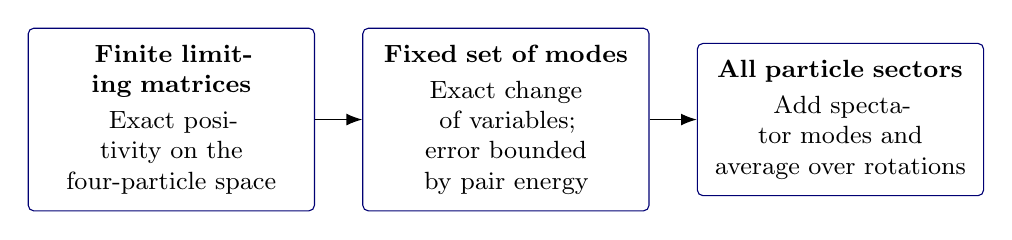
\begin{tikzpicture}[
  box/.style={draw=blue!45!black,rounded corners=2pt,align=center,
              text width=0.265\linewidth,inner sep=6pt,font=\small},
  >={Latex[length=2mm]}, node distance=6mm]
\node[box] (limit) {\textbf{Finite limiting matrices}\\[2pt]
  Exact positivity on the\\four-particle space};
\node[box,right=of limit] (local) {\textbf{Fixed set of modes}\\[2pt]
  Exact change of variables;\\error bounded by pair energy};
\node[box,right=of local] (global) {\textbf{All particle sectors}\\[2pt]
  Add spectator modes and\\average over rotations};
\draw[->] (limit) -- (local);
\draw[->] (local) -- (global);
\end{tikzpicture}

\caption{The finite-sphere comparison preserves an error relative to the
pair energy at every step. The limiting positivity is imposed only after
wedging; no invertibility of its Gram matrices is required.}
\label{fig:transfer}
\end{figure}


Section~\ref{sec:algebra} derives the normal-ordered square, and
Section~\ref{sec:spin} establishes the spin formulas.
Section~\ref{sec:squares} gives the finite comparisons.
Section~\ref{sec:transfer} proves their uniform transfer, and
Section~\ref{sec:finish} controls the tail and proves the spherical results.
Section~\ref{sec:plane} derives the planar consequence.
The exact row data, rational formulas, and complete arithmetic procedure
for the positivity checks are in Appendix~\ref{app:certificate}.

\section{Exterior algebra and the square of the interaction}
\label{sec:algebra}
Our first task is to isolate the two-, three-, and four-body terms of $H_Q^2$. The lifting notation below keeps this calculation independent of particle number.

Throughout the operator argument take $Q\ge2$; statements involving limits hold for all sufficiently large integer $Q$. We use the convention that wedges of distinct increasing orthonormal basis vectors have norm one. On
\[
 \FF_Q=\bigoplus_{n=0}^{Q+1}\bigwedge^n U_Q,
\]
let $B(v)$ be the adjoint of left wedge multiplication by $v$. Thus $B(v)$ is conjugate-linear in $v$, and
\[
 B(v\wedge w)=B(w)B(v).
\]
For an orthonormal basis $e_0,\ldots,e_Q$ of $U_Q$, write $c_j=B(e_j)$. These operators satisfy the canonical anticommutation relations, and $\norm{c_j}\le1$.

For a matrix on $\bigwedge^k U_Q$, define its lift by linear extension of
\begin{equation}\label{eq:lift}
 \LL_k(\ket v\bra w)=B(v)^\dagger B(w).
\end{equation}
This map preserves positivity, intertwines rotations, acts as the original matrix on $k$ particles, and vanishes on fewer than $k$ particles. Positivity follows by decomposing a positive matrix into a sum of rank-one positive matrices.

Put $a=Q-1$ and let $V_Q\subset\bigwedge^2 U_Q$ be the spin-$a$ summand. If $v_0,\ldots,v_{2Q-2}$ is an orthonormal basis of $V_Q$, set
\begin{equation}\label{eq:fockH}
 B_p=B(v_p),\qquad H_Q=\LL_2(\Pi_{V_Q})=\sum_{p=0}^{2Q-2}B_p^\dagger B_p.
\end{equation}
This pair-annihilator form is standard in the algebraic treatment of
pseudopotentials~\cite[Sections~II.B--D]{OrtizNussinovDukelskySeidel};
see also \cite[Equation~(2)]{ChenSeidel2015}. We verify its coefficient-one
normalization here. Its restriction to $\bigwedge^N U_Q$ is \eqref{eq:physicalH}. Indeed contraction in two specified tensor positions corresponds to $B(v)/\sqrt{\binom N2}$ under the isometric identification of wedge and antisymmetric tensor spaces; summing over the $\binom N2$ unordered pairs gives \eqref{eq:fockH}.

Define intertwining wedge maps
\[
 W_3:V_Q\otimes U_Q\longrightarrow\bigwedge^3U_Q,
 \qquad W_4:V_Q\otimes V_Q\longrightarrow\bigwedge^4U_Q,
\]
by $W_3(v\otimes u)=v\wedge u$ and $W_4(v\otimes w)=v\wedge w$. We suppress the subscript $Q$ when no confusion can result.

A finite normal-ordering calculation in the sense of Wick~\cite{Wick}
now determines the square. Only contractions between the two middle
pair operators are needed.

\begin{lemma}[Normal-ordered square]\label{lem:square}
On $\FF_Q$,
\begin{equation}\label{eq:square}
 H^2=H+\LL_3\!\left(W_3(W_3^\dagger W_3-I)W_3^\dagger\right)
       +\LL_4(W_4W_4^\dagger).
\end{equation}
\end{lemma}
\begin{proof}
In normal ordering $B_p^\dagger(B_pB_r^\dagger)B_r$, only the two inner annihilators cross the two inner creators. Two, one, or zero contractions leave two-, three-, or four-body terms, respectively. On two particles, $H=\Pi_{V_Q}$ is a projection, so the two-body coefficient is $\Pi_{V_Q}$. The term with no contractions is
\[
 \sum_{p,r}B(v_p\wedge v_r)^\dagger B(v_p\wedge v_r)
 =\LL_4(W_4W_4^\dagger).
\]
There is no extra factor of two: this sum, and the defining basis of $V_Q\otimes V_Q$, both use ordered pairs. On three particles, $H=W_3W_3^\dagger$, since $W_3$ restricted to $v_p\otimes U_Q$ is the map $B_p^\dagger$ from one to three particles. Subtracting its two-body contribution from $H^2$ therefore determines the remaining coefficient as
\[
 (W_3W_3^\dagger)^2-W_3W_3^\dagger
 =W_3(W_3^\dagger W_3-I)W_3^\dagger.
\]
Normal-ordered coefficients are determined successively by these restrictions, proving the identity on Fock space.
\end{proof}

\section{Spin coefficients and their limits}
\label{sec:spin}
The three-body comparison will use the exact spin spectrum of the wedge map. The four-body comparison will use only finitely many coupling coefficients and their limits.

The spherical pair coefficients can be expressed through angular-momentum
coupling~\cite[Section~II.C and Appendix~A]{OrtizNussinovDukelskySeidel}.
We derive the particular coefficients and fixed-deficit limits needed
here to keep their phases and normalization explicit.

We now fix $e_p$ and $v_p$ to be the normalized lowering bases of $U_Q$ and $V_Q$, respectively, with $v_0=-e_0\wedge e_1$. For spin $j$, lowering from label $p$ to $p+1$ has coefficient $\sqrt{(p+1)(2j-p)}$. Write $(s)_p=s(s-1)\cdots(s-p+1)$, with $(s)_0=1$.

\begin{lemma}[Pair coefficients]\label{lem:pair}
The coefficient of $e_i\wedge e_j$ in $v_p$, for $i<j$, vanishes unless $i+j=p+1$, and otherwise equals
\begin{equation}\label{eq:pair}
 v_p(i,j)=(i-j)\sqrt{\frac{(Q)_i(Q)_j\,p!}{Q(2Q-2)_p\,i!j!}}.
\end{equation}
For fixed $p,i,j$, its limit is
\begin{equation}\label{eq:pairstar}
 v_p^*(i,j)=(i-j)\sqrt{\frac{p!}{2^p i!j!}}\,\mathbf1_{i+j=p+1}.
\end{equation}
\end{lemma}
\begin{proof}
Apply simultaneous lowering $p$ times to $-e_0\wedge e_1$ and divide by $\sqrt{(2Q-2)_p p!}$. Expand the lowering operator binomially. Combining the two contributions to each increasing pair gives \eqref{eq:pair}. Taking the limit gives \eqref{eq:pairstar}.
The normalization can also be checked directly: the square of the
coefficient in \eqref{eq:pair} is
\[
 (i-j)^2\frac{\binom Qi\binom Qj}{Q\binom{2Q-2}{p}},
\]
and differentiating \((1+x)^Q\) gives
\[
 \sum_{i,j=0}^Q(i-j)^2\binom Qi\binom Qj x^{i+j}
 =2Qx(1+x)^{2Q-2}.
\]
Take the coefficient of \(x^{p+1}\) and halve the sum to restrict to \(i<j\).
\end{proof}

The elementary tensor product rule decomposes spins $j_1,j_2$ into one copy of each spin $j_1+j_2-z$, for $0\le z\le\min(2j_1,2j_2)$. This rule can be seen directly in the
polynomial model: at deficit $z$ the raising equation determines a highest
vector, and normalized lowering generates its $2(j_1+j_2-z)+1$
orthogonal weight vectors. Different highest spins give orthogonal
invariant subspaces, and the sum of these dimensions is
$(2j_1+1)(2j_2+1)$, exhausting the tensor product. Let $R_{3,z}$ be the corresponding projection in $V_Q\otimes U_Q$, and put
\[
 d_a=2Q-1,\qquad d_{3,z}=3Q-1-2z.
\]
For $Q\ge2$, the allowed indices are $0\le z\le Q$.

\begin{lemma}[Three-body Gram eigenvalues]\label{lem:q}
\begin{equation}\label{eq:q}
 W_3^\dagger W_3-I=\sum_{z=0}^Qq_z(Q)R_{3,z},\qquad
 q_z(Q)=(-1)^z\frac{(Q)_z}{(2Q-2)_z}
          \left(3z-1-\frac{z(z+1)}Q\right).
\end{equation}
In particular $W_3R_{3,z}=0$ for $z=0,1,3$ whenever these indices are allowed. For fixed $z$,
\begin{equation}\label{eq:qlimit}
 q_z(Q)\longrightarrow (3z-1)(-1/2)^z.
\end{equation}
\end{lemma}
\begin{proof}
Identify $V_Q\otimes U_Q$ with tensors antisymmetric in their first two positions. Then $W_3$ is $\sqrt3$ times full antisymmetrization. Its Gram operator is the compression of $I-P_{13}-P_{23}$, where $P_{ij}$ swaps tensor positions. The two swap compressions coincide, since conjugation by $P_{12}$ interchanges them and $P_{12}=-I$ on the domain. By equivariance and multiplicity-freeness they act by the same scalar $b_z$ on each spin block.

A highest vector of that block has coefficients $s_p$ on $v_p\otimes e_{z-p}$, $0\le p\le z$, satisfying
\begin{equation}\label{eq:highest-ratio}
 \frac{s_{p+1}}{s_p}=-\sqrt{\frac{(z-p)(Q-z+p+1)}{(p+1)(2Q-2-p)}}.
\end{equation}
This follows by applying the raising operator. Write
$\xi_z=\sum_{p=0}^z s_pv_p\otimes e_{z-p}$. Since
$v_0=(-e_0\otimes e_1+e_1\otimes e_0)/\sqrt2$, testing $P_{23}\xi_z$
against $v_0\otimes e_z$ tests $\xi_z$ only on the ordered triples
$(0,z,1)$ and $(1,z,0)$. Their pair labels are $z-1$ and $z$,
respectively, with the first contribution absent at $z=0$.
Substituting their pair coefficients from \eqref{eq:pair} gives
\[
 s_0b_z=\frac12\left[
 s_{z-1}\sqrt{\frac{z(Q)_z}{Q(2Q-2)_{z-1}}}
 -s_z(z-1)\sqrt{\frac{(Q)_z}{(2Q-2)_z}}\right].
\]
Here the ordered tensor coefficients of a normalized wedge include a factor $1/\sqrt2$. Iteration of \eqref{eq:highest-ratio} gives
\[
 \frac{s_z}{s_0}=(-1)^z\sqrt{\frac{(Q)_z}{(2Q-2)_z}},\qquad
 \frac{s_{z-1}}{s_0}=(-1)^{z-1}
 \sqrt{\frac{z(Q-1)_{z-1}}{(2Q-2)_{z-1}}}\quad(z\ge1).
\]
Substitution gives $q_z=-2b_z$ in the form \eqref{eq:q}. The three stated null sectors have $q_z=-1$, and \eqref{eq:qlimit} follows directly.
\end{proof}

We will repeatedly use a fixed-deficit limit of this same calculation. In a product of spins $j_1,j_2$, total lowering deficit means $T=j_1+j_2-m$, where $m$ is the total magnetic quantum number. Coefficients below are with respect to normalized monomials $X^pY^{T-p}/\sqrt{p!(T-p)!}$, and are zero outside the stated index ranges.

\begin{lemma}[Fixed-deficit coupling limit]\label{lem:coupling}
Suppose $j_1,j_2\to\infty$ and $j_2/(j_1+j_2)\to u^2$, where $0<u<1$. Put $v=\sqrt{1-u^2}$. For fixed integers $0\le z\le T$, the normalized coupled vector of spin $j_1+j_2-z$ at total lowering deficit $T$ can be chosen with real coefficients converging to the coefficients $s^{(u)}_{z,T,p}$ of
\begin{equation}\label{eq:coupling}
 \frac{(uX-vY)^z(vX+uY)^{T-z}}{\sqrt{z!(T-z)!}}.
\end{equation}
Descendants in every copy are obtained by normalized lowering, so the matching of bases between equal-spin copies is intertwining.
\end{lemma}
\begin{proof}
At $T=z$, the raising equation gives the adjacent ratio
\[
 -\sqrt{\frac{(z-p)(2j_2-z+p+1)}{(p+1)(2j_1-p)}}.
\]
With sign $(-1)^z$ at $p=0$, normalization yields the coefficients of $(uX-vY)^z/\sqrt{z!}$ in the limit. The change of variables $(X,Y)\mapsto(uX-vY,vX+uY)$ is orthogonal, so these polynomials have norm one in the normalized-monomial inner product. Normalized lowering from $T$ to $T+1$ divides the sum of the two lowering operators by
\[
 \sqrt{(T-z+1)\{2(j_1+j_2-z)-(T-z)\}}.
\]
In the limit this acts by multiplication by $(vX+uY)/\sqrt{T-z+1}$. Induction proves the statement for fixed descendants.
\end{proof}

\section{Rotational averages of explicit squares}
\label{sec:squares}
We construct a positive rotational average and compare its three- and four-body terms with those of $H_Q^2$. This section specifies the finite inequalities needed; Appendix~\ref{app:certificate} proves them by exact rational arithmetic.

Haar measure $dg$ on $SU(2)$ is normalized to have total mass one. For an operator $A$, write $A(g)=U(g)AU(g)^\dagger$, with the appropriate Fock representation. Schur averaging sends a rank-one operator on an irreducible spin-$j$ space to its trace times $I/(2j+1)$. For several equivalent copies, it acts in the same way on the spin
factor and retains the matrix between copies. Explicitly, if the
representation is $\bigoplus_j(V_j\otimes\mathbb C^{m_j})$ and $P_j$
is its spin-$j$ projection, then
\[
 \int U(g)XU(g)^\dagger\,dg
 =\bigoplus_j\frac{I_{V_j}}{2j+1}\otimes
            \operatorname{Tr}_{V_j}(P_jXP_j).
\]
Here $\operatorname{Tr}_{V_j}$ is the partial trace over the spin factor.
This follows from Schur's lemma applied to each pair of irreducible
copies, with the scalar fixed by its trace; see
\cite[Section~II.C]{BartlettRudolphSpekkens}. In particular, averaging
preserves off-diagonal entries between equivalent spin copies.

The positive-square construction belongs to the quadratic-gap approach
described in Section~\ref{sec:intro}. Fermionic positivity constraints,
normal ordering, and symmetry also appear in the quantum Hall bootstrap
of Gao et al.~\cite{GaoLanzettaLedwithWangKhalaf}, which bounds ground-state
energies. Here the explicit squares are compared with $H_Q^2-\gamma H_Q$
to control the positive excitation spectrum.

For each of the seven rows in Appendix~\ref{app:certificate}, the integer
$t_\rho$ lies in $\{0,\ldots,7\}$. Set
\[
 \mathcal S_\rho=\{(p,j)\in\mathbb Z^2:0\le p\le7,\ 0\le j\le8,\
                         0\le p+j-t_\rho\le8\}.
\]
The row specifies real coefficients $\lambda_\rho$ and
$\alpha^\rho_{pj}$ for $(p,j)\in\mathcal S_\rho$; unlisted entries are zero.
Every coefficient sum for row $\rho$ below is over $\mathcal S_\rho$.
Our comparison operator is
\begin{equation}\label{eq:F}
 K=\sum_{\rho=1}^7F_\rho^\dagger F_\rho,\qquad
 F_\rho=\lambda_\rho B_{t_\rho}
       +\sum_{(p,j)\in\mathcal S_\rho}\alpha^{\rho}_{pj}\,
                                  c_{p+j-t_\rho}^\dagger c_jB_p.
\end{equation}
Each summand of $F_\rho$ removes two particles and decreases the sum of
occupied orbital labels by $t_\rho+1$: for the second term the decrease is
$(p+1)+j-(p+j-t_\rho)=t_\rho+1$. This common weight allows the two parts
to interfere in their square, adjusting the three-body comparison at the
two-body cost $\lambda_\rho^2B_{t_\rho}^\dagger B_{t_\rho}$.
Only modes $0,\ldots,8$ occur in these auxiliary squares.

For a single row, omit $\rho$ and put $i=p+j-t$, $k=q+l-t$. Define
\[
 O_{p,j,k}=B(v_p\wedge e_j\wedge e_k)=c_kc_jB_p.
\]
Reordering $c_ic_k^\dagger=\delta_{ik}-c_k^\dagger c_i$ gives the two-, three-, and four-body terms of $F^\dagger F$:
\begin{align}
 &\lambda^2 B_t^\dagger B_t,\label{eq:normal2}\\
 &\sum_{p,j}\lambda\alpha_{pj}\left[(c_iB_t)^\dagger c_jB_p
                         +(c_jB_p)^\dagger c_iB_t\right]
   +\sum_{p,j;q,l}\alpha_{pj}\alpha_{ql}\delta_{ik}
                         (c_jB_p)^\dagger c_lB_q,\label{eq:normal3}\\
 &-\sum_{p,j;q,l}\alpha_{pj}\alpha_{ql}
                         O_{p,j,k}^\dagger O_{q,l,i}.\label{eq:normal4}
\end{align}
Let $A_2,A_3,A_4$ denote these terms, summed over rows and averaged with factor $d_a$. Thus
\begin{equation}\label{eq:Adecomp}
 \mathcal K_Q:=d_a\int K(g)\,dg=A_2+A_3+A_4,\qquad A_2=\eta H,
 \quad \eta=\sum_\rho\lambda_\rho^2.
\end{equation}

\subsection{The three-body comparison}
Before wedging, \eqref{eq:normal3} is a matrix on $V_Q\otimes U_Q$. Its nonzero entries preserve $T=p+j$, and $T\le15$. Averaging therefore gives
\begin{equation}\label{eq:A3}
 A_3=\LL_3\left(W_3\sum_{z=0}^{15}\frac{d_a}{d_{3,z}}e_z^Q R_{3,z}W_3^\dagger\right),
\end{equation}
for all sufficiently large $Q$, where $e_z^Q$ is the trace of the unaveraged matrix in that spin block. By Lemma~\ref{lem:coupling}, with $u=1/\sqrt3$, these traces converge to
\begin{equation}\label{eq:ez}
 e_z=\sum_\rho\sum_{T=\max(z,t_\rho)}^{15}
 \left[2\lambda_\rho s_{z,T,t_\rho}
                   \sum_{p+j=T}\alpha^{\rho}_{pj}s_{z,T,p}
       +\left(\sum_{p+j=T}\alpha^{\rho}_{pj}s_{z,T,p}\right)^2\right],
\end{equation}
where $s=s^{(1/\sqrt3)}$ and empty inner sums are zero. The condition $i=k$ in \eqref{eq:normal3} is exactly the equality of the two values of $T$.

The exact calculation in Appendix~\ref{app:certificate} proves
\begin{equation}\label{eq:3certificate}
 e_z<\frac32(3z-1)(-1/2)^z,
 \qquad z\in\{2,4,5,\ldots,15\}.
\end{equation}
There are finitely many strict inequalities, $d_{3,z}/d_a\to3/2$, and the omitted blocks $z=0,1,3$ are annihilated by $W_3$. Consequently, for all sufficiently large $Q$,
\begin{equation}\label{eq:A3bound}
 A_3\le\LL_3\left(W_3\sum_{z=0}^{15}q_z(Q)R_{3,z}W_3^\dagger\right).
\end{equation}

\subsection{The four-body comparison before taking limits}
Let
\[
 \widehat W:V_Q\otimes\bigwedge^2U_Q\longrightarrow\bigwedge^4U_Q
\]
be the wedge map. The second tensor factor decomposes into spins $Q-r$, with $r$ odd, $1\le r\le Q$. In its lowering bases use the sign of Lemma~\ref{lem:coupling}; at $r=1$ this is precisely the basis $v_p$.

A copy of spin $2Q-1-D$ is obtained by coupling $a=Q-1$ with $Q-r$ at deficit $D-r$. Denote its vector at total deficit $T$ by $\ket{D,T;r}_Q$. Its physical orbital-index sum is $1+T$, and it is a highest vector when $T=D$. For fixed $D,T$ and sufficiently large $Q$, the allowed copy labels are
\[
 \mathcal R_D=\{1,3,5,\ldots\}\cap[1,D],\qquad D\le T.
\]
Define the real finite-flux coefficients by
\[
 \ket{D,T;r}_Q=\sum_{\substack{p+j+k=T\\j<k}}
 S_r^Q(D,T;p,j,k)\,v_p\otimes(e_j\wedge e_k),
\]
and extend them antisymmetrically in $j,k$. By two applications of Lemma~\ref{lem:coupling}, they converge to
\begin{equation}\label{eq:S}
 S_r(D,T;p,j,k)=\sqrt2\,
 s^{(1/\sqrt2)}_{r,j+k,j}\,
 s^{(1/\sqrt2)}_{D-r,T-r,p},
\end{equation}
interpreted as zero if $r>j+k$. The formula holds for either ordering of $j,k$, by antisymmetry. It follows by applying Lemma~\ref{lem:coupling} first to the two single-particle spins and then to the two pair spins.

Only $1\le D\le23$ contribute: every unaveraged term has
\[
 T=p+j+k=q+l+i\le23.
\]
Put $d_D=4Q-1-2D$. In the coupled bases $\ket{D,T;r}_Q$, the
spin-$2Q-1-D$ block is identified with
$\mathbb C^{d_D}\otimes\mathbb C^{\mathcal R_D}$: the first factor uses the
$(T-D)$-th normalized spin descendant, and the second has basis vector
indexed by $r$. Let $E_D^Q$ be the partial trace over the spin factor of
the compression to this block of the matrix representing \eqref{eq:normal4}
before wedging, summed over rows. Schur averaging then gives, for all sufficiently large $Q$,
\begin{equation}\label{eq:A4}
 A_4=\LL_4\!\left(\widehat W
   \left[\bigoplus_{D=1}^{23}\frac{d_a}{d_D}
       (I_{d_D}\otimes E_D^Q)\right]\widehat W^\dagger\right),
\end{equation}
where the direct sum acts as zero on all other spin blocks.
For these finitely many $D$, entrywise convergence gives $E_D^Q\to E_D$, with
\begin{equation}\label{eq:E}
 (E_D)_{rs}=-\sum_\rho\sum_{\substack{p,j;q,l\\T\ge D}}
 \alpha^{\rho}_{pj}\alpha^{\rho}_{ql}
 S_r(D,T;p,j,k)S_s(D,T;q,l,i),
\end{equation}
where $i=p+j-t_\rho$, $k=q+l-t_\rho$, and $T=p+j+k$. The exact finite-flux matrix $E_D^Q$ is given by the same formula with each $S_r$ replaced by $S_r^Q$. Exchanging the two ordered entry pairs exchanges $r$ and $s$, so both matrices are real symmetric.

The target term $\LL_4(W_4W_4^\dagger)$ is obtained from the $r=1$ summand, since that summand is $V_Q\otimes V_Q$. Thus its copy matrix, in the units just used, is $(d_D/d_a)\chi$, where
\[
 \chi_{rs}=\mathbf1_{r=s=1},\qquad d_D/d_a\longrightarrow2.
\]
For even $D$, the $r=1$ coupled vector is antisymmetric under exchange
of its two spin-$a$ factors, since its coupling deficit is $D-1$.
Wedging two degree-two vectors is symmetric, so this target column then
vanishes after applying $\widehat W$. The formula with $\chi$ still
represents it exactly; we never assume that the wedged copy vectors are
independent.

Target spin blocks outside $1\le D\le23$ contribute positively and may be discarded in a lower bound.

Set
\begin{align}
 w_{Dr}^Q&=\widehat W\ket{D,D;r}_Q,\label{eq:wQ}\\
 w_{Dr}^*&=\sum_{\substack{p+j+k=D\\j<k}}
 S_r(D,D;p,j,k)\,v_p^*\wedge e_j\wedge e_k,\qquad
 (G_D)_{rs}=\ip{w_{Dr}^*}{w_{Ds}^*}.\label{eq:wstar}
\end{align}
The star is a limit label, not an adjoint. Let $W_D^*$ be the map with columns
$w_{Dr}^*$. With allowance $\eps=3\cdot10^{-6}$, the limiting comparison on
these four-particle images asks that
$W_D^*(2\chi-E_D+\eps I)(W_D^*)^\dagger$ be nonnegative.
Lemma~\ref{lem:compression} identifies this with the exact certificate
\begin{equation}\label{eq:4certificate}
 G_D(2\chi-E_D+\eps I)G_D\ge0,
 \qquad 1\le D\le23.
\end{equation}
Appendix~\ref{app:certificate} specifies and verifies it entirely by rational arithmetic.

\section{A relative error bound for finite spheres}
\label{sec:transfer}
The limiting Gram matrices have kernels, so their positivity cannot be
transferred by assuming that their ranges vary continuously.  Instead, we
compare the annihilators themselves.  An exact diagonal change of variables
reduces every error to a fixed finite family of pair-generated annihilators.
This gives an error relative to $H_Q$, uniformly on the full Fock space.

Geometry-dependent diagonal changes of occupation-number coordinates
already relate pseudopotential annihilators and their zero modes~\cite[Section~II.E]{OrtizNussinovDukelskySeidel}.
For a gap estimate, the needed additional statement is quantitative:
on a fixed set of modes the change of variables approaches the identity,
and its error is controlled by pair energy. The proof below establishes
that statement before adding spectator modes and averaging over rotations.

For the local argument, let $\FF_{\mathrm{loc}}$ be the exterior algebra
of $\mathbb C^{25}$ with orthonormal basis $e_0,\ldots,e_{24}$.
For $Q\ge24$ we identify it with the Fock space of the first 25 orbital
modes in $U_Q$. By \eqref{eq:pairstar}, each limiting pair vector $v_p^*$
with $p\le23$ lies in $\bigwedge^2\mathbb C^{25}$.
Contraction by these vectors is defined on $\FF_{\mathrm{loc}}$
by the same exterior-algebra convention as before.

\begin{lemma}[Compression and annihilator bounds]\label{lem:compression}
Let $W$ be a linear map between finite-dimensional Hilbert spaces,
$G=W^\dagger W$, and let $C$ be self-adjoint on the domain of $W$. Then
\[
 GCG\ge0\quad\Longleftrightarrow\quad WCW^\dagger\ge0.
\]
On $\FF_{\mathrm{loc}}$, for any fixed finite collection
$A_b=c_kc_jB(v_p^*)$ with $0\le p\le23$ and $0\le j,k\le24$,
\begin{equation}\label{eq:annihilatorbound}
 \sum_b\norm{A_b\psi}^2\le C_0\ip\psi{h_*\psi},
 \qquad h_*:=\sum_{p=0}^{23}B(v_p^*)^\dagger B(v_p^*),
\end{equation}
where $C_0$ depends only on the collection.
\end{lemma}
\begin{proof}
The two positivity statements both assert that the quadratic form of $C$
is nonnegative on $\ran G=\ran W^\dagger$.  For the second assertion, use
$\norm{c_kc_jB(v_p^*)\psi}\le\norm{B(v_p^*)\psi}$ and sum; one may take
$C_0$ to be the largest multiplicity of a pair label $p$.
\end{proof}

\Needspace{11\baselineskip}
\begin{lemma}[Uniform transfer]\label{lem:transfer}
For $Q\ge24$ and $1\le D\le23$, put
\[
 C_D^Q=(d_D/d_a)\chi-E_D^Q+\eps I,
 \qquad h_Q=\sum_{p=0}^{23}B_p^\dagger B_p.
\]
Assuming \eqref{eq:4certificate}, there is a scalar $\rho_Q\ge0$,
independent of $D$ and tending to zero as $Q\to\infty$, such that
\begin{equation}\label{eq:relative}
 \sum_{r,s\in\mathcal R_D}(C_D^Q)_{rs}
 B(w_{Dr}^Q)^\dagger B(w_{Ds}^Q)
 \ge-\rho_Qh_Q
\end{equation}
on the entire Fock space $\FF_Q$.
\end{lemma}
\begin{proof}
\emph{An exact change of variables.}
Take $Q\ge24$.  All annihilators in \eqref{eq:relative}, including those
in $h_Q$, involve only the modes $0,\ldots,24$. First work on
$\FF_{\mathrm{loc}}$. Define the positive diagonal operator
\[
 \Delta_Q\ket A=\left(\prod_{x\in A}d_Q(x)\right)\ket A,
 \qquad d_Q(x)=\sqrt{(Q)_x/Q^x},
\]
on each basis wedge $\ket A$.  This local Fock space is fixed as $Q$
varies.  Thus $\Delta_Q$ and $\Delta_Q^{-1}$ converge in norm to $I$;
also $0<\Delta_Q\le I$.

The pair coefficient formula \eqref{eq:pair} gives
\[
 v_p(x,y)=r_p(Q)d_Q(x)d_Q(y)v_p^*(x,y),
 \qquad r_p(Q)=\sqrt{(2Q)^p/(2Q-2)_p}\ge1.
\]
Checking the factors attached to the removed orbital labels on a basis
wedge gives the exact identities
\begin{align}
 B_p&=r_p(Q)\Delta_Q^{-1}B(v_p^*)\Delta_Q,
       \label{eq:pairconjugation}\\
 B(v_p\wedge e_j\wedge e_k)
 &=\frac{r_p(Q)}{d_Q(j)d_Q(k)}\,
   \Delta_Q^{-1}B(v_p^*\wedge e_j\wedge e_k)\Delta_Q.
       \label{eq:fourconjugation}
\end{align}
These are identities on the local Fock space, with the inverse diagonal
acting on the output particle sector.  Repeated removed labels make both
sides zero.  In particular, solving \eqref{eq:pairconjugation} for
$B(v_p^*)\Delta_Q$ and using $r_p(Q)\ge1$ and $\norm{\Delta_Q}\le1$
gives
\begin{equation}\label{eq:pairenergytransfer}
 \Delta_Q h_*\Delta_Q\le h_Q.
\end{equation}

\emph{The error is controlled by pair energy.}
Fix $D$.  Index a finite family by
$b=(p,j,k)$ with $p+j+k=D$ and $j<k$, and put
\[
 A_b=B(v_p^*\wedge e_j\wedge e_k),\qquad
 \beta_{rb}^Q=S_r^Q(D,D;p,j,k)
                \frac{r_p(Q)}{d_Q(j)d_Q(k)}.
\]
Equations \eqref{eq:wQ} and \eqref{eq:fourconjugation} yield
\[
 B(w_{Dr}^Q)=\Delta_Q^{-1}
             \left(\sum_b\beta_{rb}^QA_b\right)\Delta_Q.
\]
The coefficients are real, and Lemma~\ref{lem:coupling} gives
$\beta_{rb}^Q\to\beta_{rb}^*:=S_r(D,D;p,j,k)$.  Hence the finite
real symmetric matrices
\[
 M_Q=(\beta^Q)^TC_D^Q\beta^Q
 \quad\hbox{converge to}\quad
 M_*=(\beta^*)^T(2\chi-E_D+\eps I)\beta^*.
\]
The quadratic expression in \eqref{eq:relative} is consequently
\[
 \Delta_Q\left(\sum_{b,c}(M_Q)_{bc}
                 A_b^\dagger\Delta_Q^{-2}A_c\right)\Delta_Q.
\]
Its limiting expression before the outer diagonals is
\begin{equation}\label{eq:limitpositive}
 \sum_{b,c}(M_*)_{bc}A_b^\dagger A_c
 =\sum_{r,s}(2\chi-E_D+\eps I)_{rs}
       B(w_{Dr}^*)^\dagger B(w_{Ds}^*)\ge0.
\end{equation}
Indeed, the certificate \eqref{eq:4certificate} and
Lemma~\ref{lem:compression}, applied to the map with columns $w_{Dr}^*$,
give positivity before lifting; the lift $\LL_4$ preserves positivity.

For clarity, the perturbation estimate does not require $M_*\ge0$.
Let $R_Q$ be the block matrix with entries
\[
 (R_Q)_{bc}=(M_Q)_{bc}\Delta_Q^{-2}-(M_*)_{bc}I.
\]
Regard $R_Q$ as an operator on the Hilbert direct sum of one copy of
$\FF_{\mathrm{loc}}$ for each index $b$.  The diagonal $\Delta_Q^{-2}$
acts on the output of $A_c$, hence on the sector with four fewer particles;
using its direct sum over local sectors makes this a single operator
identity. Its norm tends to zero, since both its index set and the local
Fock space are fixed. For every vector $\phi$,
\[
 \left|\sum_{b,c}\ip{A_b\phi}{(R_Q)_{bc}A_c\phi}\right|
 \le\norm{R_Q}\sum_b\norm{A_b\phi}^2
 \le C_0\norm{R_Q}\ip\phi{h_*\phi}.
\]
Combine this estimate with \eqref{eq:limitpositive}, take
$\phi=\Delta_Q\psi$, and apply \eqref{eq:pairenergytransfer}.  This
proves \eqref{eq:relative} on the local Fock space with a coefficient
tending to zero.  Taking a maximum over the fixed set $1\le D\le23$
gives a common $\rho_Q$.

\emph{Additional particles are spectators.}
Order the 25 local modes before all other modes in the Fock
factorization.  Under the isometry that sends a local wedge tensored with a spectator
wedge to their ordered product, each $c_j$ with $j\le24$ is its local
annihilator tensored with the identity. The fermionic parity factor belongs
to annihilators in the later spectator modes, which do not occur here.
Thus every operator in \eqref{eq:relative} acts on the local factor alone.
Tensoring the local inequality with the identity proves
it on $\FF_Q$, with the same $\rho_Q$, regardless of the number of
occupied modes outside this factor.
\end{proof}

The allowance $\eps I$ in the certificate must also be paid for in pair
energy.  Here it is useful to sum over the orthonormal highest vectors
\emph{before} estimating their wedges.  Bessel's inequality then avoids
an extra factor equal to the number of spin copies.

\begin{proposition}[Four-body estimate]\label{prop:A4}
For the coefficients in Appendix~\ref{app:certificate},
\begin{equation}\label{eq:A4bound}
 A_4\le\LL_4(W_4W_4^\dagger)+(1222\eps+o(1))H,
 \qquad Q\to\infty,
\end{equation}
uniformly on $\FF_Q$.
\end{proposition}
\begin{proof}
Haar averaging the matrix unit
$\ket{D,D;r}_Q\bra{D,D;s}_Q$ gives the corresponding copy matrix unit
tensored with the spin identity, divided by $d_D$.  Therefore, on the
retained spin blocks, the target minus $A_4$, with the $\eps I$ allowance
added, is
\[
 d_a\sum_{D=1}^{23}\int\sum_{r,s}(C_D^Q)_{rs}
 B(w_{Dr}^Q(g))^\dagger B(w_{Ds}^Q(g))\,dg.
\]
Lemma~\ref{lem:transfer}, conjugated by each rotation, bounds this below
by $-o(1)H$, because Schur averaging gives
\[
 d_a\int h_Q(g)\,dg=24H.
\]
The number of retained blocks is fixed, so this error remains uniform
in particle number.

To bound the allowance, fix $D$ and write
\[
 \ket{D,D;r}_Q
   =\sum_{\substack{p+j+k=D\\j<k}}S_{rb}^Q\,
                     v_p\otimes(e_j\wedge e_k),
 \qquad b=(p,j,k).
\]
The uncoupled vectors on the right are orthonormal.  So are the highest
vectors on the left: distinct $r$ belong to orthogonal spin summands of
the second pair factor.  Thus $S^Q(S^Q)^T=I$.  Apply the contraction
$S^Q\otimes I$ to the Hilbert-space-valued vector
$(c_kc_jB_p\psi)_b$.  It follows that
\[
 \sum_{r\in\mathcal R_D}\norm{B(w_{Dr}^Q)\psi}^2
 \le\sum_{\substack{p+j+k=D\\j<k}}\norm{c_kc_jB_p\psi}^2
 \le\sum_{\substack{p+j+k=D\\j<k}}\norm{B_p\psi}^2.
\]
This uses orthogonality before wedging; the vectors $w_{Dr}^Q$ themselves
need not be orthogonal.  The number of triples on the right is
\[
 n_D=\sum_{n=1}^D\left\lceil\frac n2\right\rceil
     =\left\lfloor\frac{(D+1)^2}{4}\right\rfloor.
\]
Conjugate by rotations and integrate.  Each pair norm contributes
$\ip\psi{H\psi}/d_a$, so the total allowance is bounded by
\[
 \eps\sum_{D=1}^{23}n_DH
 =\eps\left(\sum_{m=1}^{12}m^2+
                 \sum_{m=1}^{11}m(m+1)\right)H
 =1222\eps H.
\]
The discarded target spin blocks are positive.  Removing the allowance
therefore proves \eqref{eq:A4bound}.
\end{proof}

\section{The tail estimate and the gap}
\label{sec:finish}
The finite comparisons are now in place. We first bound all remaining three-body blocks by a summable multiple of $H_Q$, then identify the zero mode at Laughlin flux.

\begin{lemma}[Three-body tail]\label{lem:tail}
For sufficiently large $Q$,
\begin{equation}\label{eq:tailbound}
 \LL_3\left(W_3\sum_{z=16}^Qq_z(Q)R_{3,z}W_3^\dagger\right)
 \ge-\delta_QH,
\end{equation}
where
\begin{equation}\label{eq:delta}
 \delta_Q=\sum_{\substack{17\le z\le Q\\z\text{ odd}}}
       \frac{d_{3,z}}{d_a}|q_z(Q)|(z+1),\qquad
 \delta_Q\longrightarrow\frac{61}{4096}.
\end{equation}
\end{lemma}
\begin{proof}
For $16\le z\le Q$, the bracket in \eqref{eq:q} is positive, since it is at least $2z-2$. Thus only odd $z$ contribute negatively. A normalized highest vector of $R_{3,z}$ is $\sum_{p=0}^zs_pv_p\otimes e_{z-p}$. Its orbit resolves that spin projector with factor $d_{3,z}$. After wedging and lifting, its quadratic form is
\[
 \norm{\sum_{p=0}^zs_pc_{z-p}(g)B_p(g)\psi}^2
 \le\sum_{p=0}^z\norm{B_p(g)\psi}^2.
\]
Averaging each summand proves \eqref{eq:tailbound} with \eqref{eq:delta}.

For $Q\ge4$, the ratios in $(Q)_z/(2Q-2)_z$ are nonincreasing, so
\[
 \frac{(Q)_z}{(2Q-2)_z}\le\left(\frac Q{2Q-2}\right)^z
 \le(2/3)^z,\qquad \frac{d_{3,z}}{d_a}\le2.
\]
The summands, extended by zero for $z>Q$, are therefore dominated by
$6z(z+1)(2/3)^z$. Dominated convergence and \eqref{eq:qlimit} give
\[
 \lim_{Q\to\infty}\delta_Q
 =\frac32\sum_{z=17,19,\ldots}(3z-1)(z+1)2^{-z}
 =\frac{61}{4096}.
\]
For the last identity, write $z=17+2m$. Then
$(3z-1)(z+1)=900+208m+12m^2$, while the sums of $4^{-m}$,
$m4^{-m}$, and $m^24^{-m}$ are $4/3$, $4/9$, and $20/27$,
respectively. Multiplication by $(3/2)2^{-17}$ gives $61/4096$.
\end{proof}

\begin{proof}[Proof of Theorem~\ref{thm:fock}]
Combine Lemma~\ref{lem:square}, \eqref{eq:Adecomp}, \eqref{eq:A3bound}, Proposition~\ref{prop:A4}, and Lemma~\ref{lem:tail}. They give
\[
 H^2\ge d_a\int K(g)\,dg+
       (1-\eta-\delta_Q-1222\eps-o(1))H.
\]
The integral is positive. The certificate gives
\[
 \eta=\frac{93527408868499}{10^{14}},\qquad\eps=\frac3{10^6},
\]
so the coefficient tends to
\begin{equation}\label{eq:finalmargin}
 1-\frac{93527408868499}{10^{14}}-\frac{61}{4096}
   -1222\frac3{10^6}
 =\gamma_*=\frac{4616733319001}{10^{14}}>\frac1{25}.
\end{equation}
The limit in \eqref{eq:finalmargin} is $\gamma_*$. For each fixed $0<\gamma<\gamma_*$, the coefficient therefore exceeds $\gamma$ for all sufficiently large $Q$. Every convergence threshold is independent of particle number, proving the assertion on $\FF_Q$.
\end{proof}

We now recover the known unique zero mode of Haldane's spherical
parent Hamiltonian~\cite[p.~606, Equations~(6)--(7)]{Haldane}.
The elementary divisibility proof also fixes the exact flux at which the
kernel is a line.

\begin{lemma}[Kernel at Laughlin flux]\label{lem:kernel}
For $N\ge2$ and $Q=3(N-1)$, the kernel of $H_{N,Q}$ is the line spanned by $\Psi_{\mathrm L,N}$.
\end{lemma}
\begin{proof}
Realize $U_Q$ as the homogeneous polynomials of degree $Q$ in spinor coordinates $(u,v)$. Write $b_{ij}=u_iv_j-u_jv_i$. The pair-spin $Q-r$ summand has highest polynomial
\[
 b_{ij}^{\,r}u_i^{Q-r}u_j^{Q-r}.
\]
Since $b_{ij}$ is invariant under simultaneous rotations of the pair, every vector in this summand is divisible by $b_{ij}^r$. Exchange of the pair has parity $(-1)^r$, so antisymmetric pair states have odd $r$.

If $H_{N,Q}\Psi=0$, then, in the ambient tensor space,
\[
 0=\ip\Psi{H_{N,Q}\Psi}=\sum_{i<j}\norm{P_{ij}^{(1)}\Psi}^2.
\]
Thus $P_{ij}^{(1)}\Psi=0$ for every pair. Expanding in the other particles' monomials, the remaining pair sectors all have odd $r\ge3$. Thus $b_{ij}^3$ divides $\Psi$ for every $i<j$. Each bracket $b_{ij}=v_ju_i-u_jv_i$ is primitive as a polynomial in $u_i$, since $v_j$ and $u_jv_i$ are coprime, and is linear over the fraction field of the other variables. Gauss's lemma therefore makes it irreducible in the polynomial ring. Brackets for distinct unordered pairs are nonassociate. They are consequently relatively prime. Unique factorization implies
\[
 \prod_{i<j}b_{ij}^3\mid\Psi.
\]
This product has degree $3(N-1)=Q$ in each particle's spinor variables, exhausting the multidegree of $\Psi$; the quotient is constant.

Conversely, $\Psi_{\mathrm L,N}$ is antisymmetric. Its factor $b_{ij}^3$ leaves pair degrees $Q-3$ in each spinor, whose maximum total pair spin is $Q-3$. Multiplication by the invariant bracket cannot introduce spin $Q-1$. Hence every pair projector annihilates $\Psi_{\mathrm L,N}$.
\end{proof}

\begin{proof}[Proof of Corollary~\ref{thm:main}]
Apply Theorem~\ref{thm:fock} with $\gamma=1/25$. On each particle sector,
the spectral theorem gives
\[
 H_{N,Q}\ge\frac1{25}\bigl(I-P_{\ker H_{N,Q}}\bigr)
\]
once $Q$ exceeds the common threshold. Take $Q=3(N-1)$ and apply
Lemma~\ref{lem:kernel}. Choosing $N_0$ so that $3(N_0-1)$ exceeds the
threshold proves the claim.
\end{proof}

The following comparison specializes the recursive spectral relations of
Lemm, Nachtergaele, Warzel, and Young
\cite[arXiv v1, Theorem~2.1(I), Lemma~2.3, and (2.10)]{LemmNachtergaeleWarzelYoung2026Recursive}.

\begin{corollary}[Charge versus neutral gap at fixed flux]\label{cor:charge-neutral}
For \(N\ge2\), fix \(Q_N=3(N-1)\) and write
\(E_0(n;Q_N)=\min\operatorname{spec}H_{n,Q_N}\) for the coefficient-one
interaction \eqref{eq:physicalH}.  Let \(\operatorname{Gap}_N\) be the
first positive eigenvalue of \(H_{N,Q_N}\), its neutral gap.
The particle-number charge gap at this same flux,
\[
 \Delta_N=E_0(N+1;Q_N)+E_0(N-1;Q_N)-2E_0(N;Q_N),
\]
satisfies
\[
 \Delta_N=E_0(N+1;Q_N)
       \ge\frac{N}{N-1}\operatorname{Gap}_N>0.
\]
In particular, \(\Delta_N\ge N/[25(N-1)]\) for \(N\ge N_0\), with
\(N_0\) as in Corollary~\ref{thm:main}.
\end{corollary}

\begin{proof}
All three sectors are nonempty since \(N+1\le\dim U_{Q_N}=3N-2\).
Lemma~\ref{lem:kernel} gives \(E_0(N;Q_N)=0\) and a one-dimensional
ground space.  The \(N\)-particle sector has dimension greater than one,
so \(\operatorname{Gap}_N>0\).
For a nonzero Laughlin vector \(\Psi\), each pair annihilator \(B_p\)
commutes with every \(c_j\), while
\(\sum_j\|c_j\Psi\|^2=N\|\Psi\|^2\).  Thus some \(c_j\Psi\) is a nonzero
\((N-1)\)-particle zero mode, giving \(E_0(N-1;Q_N)=0\).
The divisibility argument in Lemma~\ref{lem:kernel} excludes a zero mode
in the \((N+1)\)-particle sector: the required product of cubed brackets
would have degree \(3N>Q_N\) in each particle variable.

Let \(P_n\) project onto the lowest-energy eigenspace of \(H_{n,Q_N}\),
and define the overlap operator on the \((N+1)\)-particle sector by
\[
 \mathcal G_N=P_{N+1}\left(\sum_{j=0}^{Q_N}c_j^\dagger P_Nc_j\right)P_{N+1}.
\]
Here \(P_{N+1}\) projects onto a positive-energy ground eigenspace.
For the pure two-body fermionic form \eqref{eq:fockH}, the cited
Theorem~2.1(I), with \(m_0=m_1=2\), gives
\[
 E_0(N+1;Q_N)\ge\frac{N+1}{N-1}E_0(N;Q_N)
   +\frac{N+1-\|\mathcal G_N\|}{N-1}\operatorname{Gap}_N.
\]
The cited Lemma~2.3 gives \(\|\mathcal G_N\|\le\operatorname{rank}P_N=1\).
Since \(E_0(N;Q_N)=0\), this yields
\(E_0(N+1;Q_N)\ge N\operatorname{Gap}_N/(N-1)\).
The two zero energies give the asserted second difference, and
Corollary~\ref{thm:main} supplies the final uniform bound.
\end{proof}

\section{A planar corollary}
\label{sec:plane}

The full-Fock-space estimate also gives a gap on the plane. We use the
analytic lowest-Landau-level representation described by Girvin and
Jach~\cite[Section~II]{GirvinJach}, with Gaussian scale fixed below.
Let
$\mathcal B$ be the Bargmann space of entire functions with norm
\[
 \|f\|_{\mathcal B}^2=\frac1\pi\int_{\mathbb C}|f(z)|^2e^{-|z|^2}\,d^2z,
 \qquad e_j(z)=\frac{z^j}{\sqrt{j!}}.
\]
Multiplication by $\pi^{-1/2}e^{-|z|^2/2}$ identifies this space unitarily
with the planar lowest Landau level at magnetic field $2$; changing magnetic
length is a unitary dilation.
For a pair of coordinates set $w=(z_1-z_2)/\sqrt2$ and
$Z=(z_1+z_2)/\sqrt2$.  Let $P^{(1)}$ be the orthogonal projector onto
relative degree one, with no restriction on the degree in $Z$, and put
\[
 H_N^{\mathrm{pl}}=\left.\sum_{1\le i<j\le N}P_{ij}^{(1)}
                         \right|_{\bigwedge^N\mathcal B}.
\]
Thus each pair projector has coefficient one, as on the sphere.

\begin{corollary}[Planar spectral gap]\label{cor:plane}
For every $N\ge2$, the untruncated planar Hamiltonian satisfies
\[
 (H_N^{\mathrm{pl}})^2\ge\gamma_* H_N^{\mathrm{pl}},
\]
where $\gamma_*$ is the constant in Theorem~\ref{thm:fock}.
Equivalently, if $P_{0,N}^{\mathrm{pl}}$ projects onto its kernel, then
$H_N^{\mathrm{pl}}\ge\gamma_*(I-P_{0,N}^{\mathrm{pl}})$.
The constant is independent of both particle number and total angular
momentum.  In particular, the case $\ell=3$ of the spectral gap conjecture
in \cite[Conjecture~A.1]{Rougerie} holds, in its pair-projector normalization.
\end{corollary}
\begin{proof}
The coordinate change $(z_1,z_2)\mapsto(w,Z)$ is unitary for the
Bargmann inner product.  Consequently the vectors
$wZ^p/\sqrt{p!}$, $p\ge0$, form an orthonormal basis of the relative-degree-one
subspace.  Their coefficients in the normalized wedge basis are
\[
 v_p^{\mathrm{pl}}(i,j)
   =(i-j)\sqrt{\frac{p!}{2^p i!j!}}\,\mathbf1_{i+j=p+1},
 \qquad i<j.
\]
Indeed, expanding $(z_1-z_2)(z_1+z_2)^p$
first gives the coefficient in the tensor basis; passage to the normalized
antisymmetric wedge multiplies it by $\sqrt2$.  These are exactly the
limits in \eqref{eq:pairstar}.  The second-quantized pair-projector identity
therefore gives
$H_N^{\mathrm{pl}}=\sum_{p\ge0}B(v_p^{\mathrm{pl}})^\dagger B(v_p^{\mathrm{pl}})$
on antisymmetric polynomials.

Fix $N$ and a total degree $L$.  The corresponding homogeneous subspace
has the finite orthonormal basis
\[
 e_{i_1}\wedge\cdots\wedge e_{i_N},\qquad
 0\le i_1<\cdots<i_N,\qquad \sum_{k=1}^N i_k=L.
\]
For $Q\ge\max\{L,N-1,2\}$ this is also the entire spherical subspace of total
lowering deficit $L$, under the identification of normalized one-particle
bases.  Both Hamiltonians preserve this subspace: a pair is annihilated
and created with the same sum of orbital labels.  Only $p+1\le L$
can contribute.  The finitely many matrix entries of the spherical
restriction therefore converge to those of the planar restriction by
\eqref{eq:pair}--\eqref{eq:pairstar}; the convergence is in operator norm.

Fix $0<\gamma<\gamma_*$.  Theorem~\ref{thm:fock} gives
$H_Q^2\ge\gamma H_Q$ for all sufficiently large $Q$.
Restrict to the invariant block just described and let $Q\to\infty$.
Norm convergence passes through the square and gives
$(H_N^{\mathrm{pl}})^2\ge\gamma H_N^{\mathrm{pl}}$ on that block.
Now let $\gamma\uparrow\gamma_*$; the cone of positive matrices is closed,
so the same inequality holds at $\gamma_*$.  The limit $Q\to\infty$ is taken
separately for each fixed $\gamma$, allowing the flux threshold to depend
on $\gamma$.  Here $N$ and $L$ were arbitrary, and the resulting constant is the
same for all of them.

Finally, $\bigwedge^N\mathcal B$ is the Hilbert direct sum of its homogeneous
subspaces, and $0\le H_N^{\mathrm{pl}}\le\binom N2 I$.  The block inequalities
thus extend by continuity to the whole space.  The spectral theorem gives
the asserted gap.  Restriction to total degrees
$L\le3N(N-1)/2$ gives exactly the sector in the cited conjecture for
$\ell=3$.
\end{proof}

\appendix
\section{The finite rational certificate}
\label{app:certificate}
This appendix specifies the seven rows and all arithmetic needed to verify
\eqref{eq:3certificate} and \eqref{eq:4certificate}. Starting from the integer
rows in Section~\ref{app:rows}, evaluate the rational three-body traces in
Section~\ref{app:three-arithmetic} and the rational four-body matrices in
Section~\ref{app:four-arithmetic}. The margin and coefficient-sign tables in
those sections record the resulting checks. The formulas below determine
every value using only integers and rational numbers.

\subsection{Row data}
\label{app:rows}
Let $P=10^7$. The first two numbers of each row are $t$ and $\ell=P\lambda$. An entry $pj:a$ specifies the integer $a_{pj}$, with $p$ and $j$ parsed as separate single-digit labels; omitted entries are zero. Continuation lines belong to the preceding row. Define
\begin{equation}\label{eq:alphadata}
 \alpha_{pj}=\frac{a_{pj}}P
       \sqrt{\frac{2^p\binom{p+j}{p}}{2^t\binom{p+j}{t}}}
 =\frac{a_{pj}}P\sqrt{\frac{2^{p-t}t!(p+j-t)!}{p!j!}}.
\end{equation}
Every nonzero entry has $0\le p+j-t\le8$.
\par\noindent\begin{minipage}{\linewidth}
\lstinputlisting{../verification/rows.txt}
\end{minipage}\par
\smallskip
\noindent In particular $P^2\eta=\sum_\rho\ell_\rho^2=93527408868499$.

\subsection{Three-body arithmetic}
\label{app:three-arithmetic}
For $c\in\{1,2\}$, an integer $T\ge0$, and integers $z,p$, define
\begin{equation}\label{eq:U}
 \mathsf U(c,z,T,p)=
 \sum_{h=\max(0,p+z-T)}^{\min(p,z)}
 (-1)^{z-h}\binom zh\binom{T-z}{p-h}c^{p-h},
\end{equation}
and set it to zero if $z$ or $p$ lies outside $[0,T]$. Expanding \eqref{eq:coupling} gives
\[
 s^{(1/\sqrt3)}_{z,T,p}=\mathsf U(2,z,T,p)
 \sqrt{\frac{2^z\binom Tz}{3^T2^p\binom Tp}}.
\]
Substitution in \eqref{eq:ez} and \eqref{eq:alphadata} cancels all radicals:
\begin{equation}\label{eq:erational}
 P^2e_z=\sum_\rho\sum_{T=\max(z,t_\rho)}^{15}
 \frac{2^z\binom Tz}{3^T2^{t_\rho}\binom T{t_\rho}}
 X_{\rho,T}\left(X_{\rho,T}+2\ell_\rho\mathsf U(2,z,T,t_\rho)\right),
\end{equation}
where $X_{\rho,T}=\sum_{p+j=T}a^\rho_{pj}\mathsf U(2,z,T,p)$, with value zero on empty levels. For each $z\in\{2,4,5,\ldots,15\}$, evaluate \eqref{eq:erational} and form the exact rational margin
$m_z=\frac32(3z-1)(-1/2)^z-e_z$. Write $10^6m_z=n_z/d_z$ with integers $n_z,d_z$ and $d_z>0$. Integer division gives the floors $\lfloor n_z/d_z\rfloor$ listed below:
\begin{center}
\begin{tabular}{rrrrrrrrrrrrrr}
\toprule
$z$&2&4&5&6&7&8&9&10&11&12&13&14&15\\
\midrule
floor&1298313&211317&249&250&249&250&250&250&249&250&250&6470&250\\
\bottomrule
\end{tabular}
\end{center}
All are positive, proving \eqref{eq:3certificate}.

\subsection{Four-body arithmetic}
\label{app:four-arithmetic}
Fix $1\le D\le23$; all copy indices below lie in $\mathcal R_D$. Put
\[
 u_r=\frac1{r!(D-r)!},\qquad
 (E_D)_{rs}=\sqrt{u_ru_s}\,Y_{rs},\qquad
 (G_D)_{rs}=\sqrt{u_ru_s}\,Z_{rs}.
\]
The matrices $Y,Z$ are rational. Define
\[
 \mathsf V_r(D,T;p,j,k)=
 \mathsf U(1,r,j+k,j)\mathsf U(1,D-r,T-r,p),
\]
with value zero for $r>j+k$. Two applications of \eqref{eq:coupling} give
\begin{equation}\label{eq:Srational}
 S_r(D,T;p,j,k)=\mathsf V_r(D,T;p,j,k)
 \sqrt{2^{1-(j+k)-T+r}\frac{j!k!p!\,u_r}{(T-D)!}}.
\end{equation}
Therefore
\begin{equation}\label{eq:Yrational}
 \begin{split}
 P^2Y_{rs}=-\sum_\rho\sum_{\substack{p,j;q,l\\T\ge D}}
 &a^\rho_{pj}a^\rho_{ql}\,
 \mathsf V_r(D,T;p,j,k)\mathsf V_s(D,T;q,l,i)\\
 &\times2^{1-2T+p+q-t_\rho+(r+s)/2}
       \frac{i!k!t_\rho!}{(T-D)!},
 \end{split}
\end{equation}
where $i=p+j-t_\rho$, $k=q+l-t_\rho$, and $T=p+j+k$. Both entry sums are ordered. To verify the cancellation, multiply the two factors in \eqref{eq:Srational} by the two factors \eqref{eq:alphadata}; the factorial product under the combined square root is
$(t_\rho!i!k!)^2u_ru_s/((T-D)!)^2$.
Using $j+k=T-p$ and $l+i=T-q$, its power of two has exponent
$2+2p+2q-2t_\rho-4T+r+s$. Taking the positive square root and
removing $\sqrt{u_ru_s}$ gives exactly the displayed factor.

For an increasing quadruple $A$ of nonnegative indices with sum $D+1$, put $f(A)=\prod_{b\in A}b!$. If $(x,y,j,k)$ lists its elements, let $\sigma(x,y,j,k)$ be the sign of sorting this list into increasing order. In each summand below put $p=x+y-1$, and define
\begin{equation}\label{eq:Lrational}
 L_r(A)=2^{(1-2D+r)/2}
 \sum_{\substack{x<y\text{ in }A\\\{j,k\}=A\setminus\{x,y\},\ j<k}}
 \sigma(x,y,j,k)(x-y)\,p!j!k!\,
 \mathsf V_r(D,D;p,j,k).
\end{equation}
Combining \eqref{eq:pairstar} and \eqref{eq:Srational}, the coefficient of $w_{Dr}^*$ on the Slater wedge $A$ is $\sqrt{u_r/f(A)}L_r(A)$. Thus
\begin{equation}\label{eq:Zrational}
 Z_{rs}=\sum_{\substack{A\text{ increasing quadruple}\\\sum_{b\in A}b=D+1}}
                   \frac{L_r(A)L_s(A)}{f(A)}.
\end{equation}
All exponents of two in these formulas are integers, since $r,s$ are odd.

Let $D_u=\diag(u_r)$ and $D_{\sqrt u}=\diag(\sqrt{u_r})$. The matrix in \eqref{eq:4certificate} equals $D_{\sqrt u}MD_{\sqrt u}$, where
\begin{equation}\label{eq:M}
 M=ZBZ,\qquad
 B=\diag\bigl((2\mathbf1_{r=1}+\eps)u_r\bigr)-D_uYD_u.
\end{equation}
Thus it suffices to check $M\ge0$ using rational arithmetic. This
congruence uses only the positive diagonal $D_{\sqrt u}$; it does not
invert $G_D$ or presume that its columns are independent.

To check positivity for each $D=1,\ldots,23$, form $Y$ and $Z$ from
\eqref{eq:Yrational} and \eqref{eq:Zrational}, then form $B$ and $M$ from
\eqref{eq:M}, using $\eps=3/10^6$. All sums range over the printed rows and
the finite index sets specified above. Compute with exact fractions
throughout. If $d=|\mathcal R_D|$, initialize $J=I_d$. For
$b=1,\ldots,d$, compute in order
\begin{equation}\label{eq:recurrence}
 X=MJ,\qquad c_b=\frac{\tr X}{b},\qquad J=c_bI_d-X.
\end{equation}
This is the Leverrier--Faddeev recurrence applied to $-M$;
see \cite{HouConference}. It gives
$\det(xI+M)=x^d+c_1x^{d-1}+\cdots+c_d$. For example, this recurrence follows by multiplying the polynomial adjugate of $xI+M$ by $xI+M$ and comparing coefficients, together with the derivative-of-determinant trace identity. Exact evaluation of \eqref{eq:U}, \eqref{eq:Yrational}, \eqref{eq:Lrational}, \eqref{eq:Zrational}, and \eqref{eq:recurrence} gives:
\begin{center}
\begin{tabular}{rl@{\qquad}rl@{\qquad}rl}
\toprule
$D$&signs&$D$&signs&$D$&signs\\
\midrule
1&\texttt{0}&9&\texttt{++000}&17&\texttt{++++++000}\\
2&\texttt{0}&10&\texttt{+0000}&18&\texttt{+++++0000}\\
3&\texttt{00}&11&\texttt{+++000}&19&\texttt{+++++++000}\\
4&\texttt{00}&12&\texttt{++0000}&20&\texttt{++++++0000}\\
5&\texttt{+00}&13&\texttt{++++000}&21&\texttt{++++++++000}\\
6&\texttt{000}&14&\texttt{+++0000}&22&\texttt{+++++++0000}\\
7&\texttt{+000}&15&\texttt{+++++000}&23&\texttt{+++++++++000}\\
8&\texttt{+000}&16&\texttt{++++0000}&&\\
\bottomrule
\end{tabular}
\end{center}
The signs list the coefficients after the leading $1$, in descending degree.
For each computed coefficient, choose a positive denominator and inspect
its integer numerator: \texttt{+} denotes a positive numerator and
\texttt{0} denotes zero. We use the characteristic-coefficient positivity test for symmetric
matrices~\cite[Theorem~5]{PeyrlParrilo}. Every coefficient is nonnegative,
so $\det(xI+M)>0$ for $x>0$. Since $M$ is real symmetric, a negative eigenvalue would give a positive root of this polynomial. Therefore $M\ge0$, proving \eqref{eq:4certificate}.

\begin{remark}[Nature of the certificate]
The data above certify fixed spin-matrix inequalities. The positive comparison operator is a sum of squares by construction. No many-particle finite-size spectrum, numerical extrapolation, or assumed plasma property enters the argument. The exact equalities and inequalities in this appendix can be verified by a finite calculation using only integers and rational numbers.
\end{remark}

\bibliographystyle{plain}
\bibliography{references}
\end{document}
